\documentclass[11pt]{article}
\usepackage[a4paper,margin=1in]{geometry}
\usepackage[T1]{fontenc}
\usepackage[utf8]{inputenc}
\usepackage{lmodern}
\usepackage{microtype}
\usepackage{amsmath,amssymb}
\usepackage{graphicx}
\usepackage{booktabs}
\usepackage{xcolor}
\usepackage{hyperref}
\usepackage[numbers,sort&compress]{natbib}
\usepackage{caption}
\hypersetup{colorlinks=true,linkcolor=blue!50!black,citecolor=blue!50!black,urlcolor=blue!50!black}
\captionsetup{font=small,labelfont=bf}
\graphicspath{{figures/}}
\setlength{\parskip}{0.25em}
\emergencystretch=1em
\newcommand{\ci}[2]{[#1,\,#2]}
% Zenodo DOIs, filled at deposit time: this version (v4) and the evidence deposit
% (run data and dated pre-registration entries). Date of the version: update if
% the deposit is published on another day.
\newcommand{\thisdoi}{10.5281/zenodo.23163708}
\newcommand{\evidencedoi}{10.5281/zenodo.23163299}
\newcommand{\versiondate}{5 October 2026}

\title{What State-Space Injection Buys in Open-Ended Generation,\\ and What It Costs}
\author{Roberto I. Ono Filho\\ Independent researcher\\
\texttt{ono.roberto@gmail.com} \quad ORCID \href{https://orcid.org/0009-0006-8650-629X}{0009-0006-8650-629X}}
\date{\small Version 4, \versiondate{} (Zenodo, doi:\href{https://doi.org/\thisdoi}{\thisdoi}; concept record \href{https://doi.org/10.5281/zenodo.22280784}{10.5281/zenodo.22280784}): corrections, listed under ``Changes in version 4'' at the end. Version 3, 11 September 2026: typography only. Version 2, 11 September 2026: revision after the fifth round of review by AI reviewer agents (the text arm re-judged at offset $+0$; the fully matched contrast as the headline). Version 1, 3 September 2026, under the title ``Pulsed, Not Pressed: \ldots''.}

\begin{document}
\maketitle

\begin{abstract}
A research program on machine novelty has intervened at three depths of
a language model (the token distribution, the context, and the
weights) and measured the limit of each. This paper opens the fourth,
the residual stream during live generation, and asks what an
intervention there buys against the written word. We inject
model-derived concept directions as guarded, pulsed translations into
Qwen3-8B-Base and measure the result under a judge-blind protocol: a
blind judge scores surprise, connection and coherence on windows of
generated-only text, paired over premises, every confirmatory analysis
pre-registered. (i)~Against text interruption, the program's flagship
prompt-side intervention, the guarded pulse trails in judged
surprise at every matched offset (thirty premises, three offsets judged
in both arms: $-0.73$ \ci{-1.19}{-0.27}; at the end of the intervention
itself the written subject scores $1.2$ points higher) and trails in
connection and coherence; the pre-registered cell average, which
contains the pulse's best offset and no text counterpart, had shown
equivalence within $\pm0.75$, with its coherence guard failing.
(ii)~A meaningful direction carries the effect: sham pulses in random
or shuffled directions displace the state more and produce less, and a
blind manipulation check finds the injected subject in the text, about
half as often as when written. (iii)~Pulsing for 32 tokens every 300
beats pressing at equal per-token dose, where the pressed arm
degenerates; at equal integrated dose the difference is not
significant. (iv)~The surprise pattern replicates in-family at 14B. The
verdict on inference-time fertility: latent injection buys a
content-specific gain in judged novelty that stays below the written
word's, at a coherence cost that halves within 150 tokens and does not
vanish. We release the code, the run data with every judge verdict, and
the dated pre-registration entries.
\end{abstract}

\section{Introduction}
\label{sec:intro}

Can a language model produce something genuinely new, and which
interventions actually help? A sequence of studies has approached this
question one substrate at a time, under a fixed measurement discipline:
judged surprise, connection and coherence on windows containing only
generated text (so that the judge can never be shown the intervention
itself)~\citep{ono2026interrupting}, and, in verifiable domains, an
exact evaluator with classical baselines~\citep{ono2026mass}. At the
\emph{token} level, anti-probable sampling bought only surface novelty.
At the \emph{context} level, periodically interrupting a habituated
stream with a new subject raised judged surprise by 1.2 to 1.4 points
over habituation alone, on fresh generated-only windows, the flagship
positive of the program, while constant pressure (a continuity
connective) was worse than nothing \citep{ono2026interrupting}. At the \emph{weight} level, consolidating
a model's own verified findings moved the mean toward the known good
and never beyond it, paying for mass with tails \citep{ono2026mass};
in verified search, operator packages composed additively and stalled
at plateaus every arm shared, the flagship one read in the companion's
current version as the resolution limit of the verifier's grid rather
than a construction-family boundary \citep{ono2026operator}. Between the context and the token sits the object
none of these touched: the residual stream $h_\ell(t)$, the thought
in progress. Recent work shows, under stated assumptions and empirically on three
models, that steered activations reach states no discrete prompt
reaches~\citep{mishra2026nonsurjective}, but leaves their \emph{value}
untested. Activation steering has mostly been a control tool (removing
behaviors, enforcing
styles~\citep{turner2023actadd,panickssery2023caa,li2023iti,zou2023repe,arditi2024refusal}),
and where it has been pointed at open-ended generation or at
creativity \citep{dathathri2020pplm,olson2024creativity,schapiro2026creativityneuro}
it was not compared with a prompt-matched rival under a judge that
never sees the intervention (a \emph{judge-blind} protocol, which is
what we mean by deception-resistant below).

This paper does that. Its contributions:

\begin{enumerate}
\item \textbf{An instrument}: guarded, pulsed translations along
  model-derived directions in the residual stream
  (\S\ref{sec:instrument}), a dimensionless dose unit and the logged
  effective displacement of every burst; dual MLX/PyTorch backends,
  bit-identical on the operators. Other operators of the same family
  (a plane rotor, a projection, repulsion from a moving mean) were
  tried and are reported as secondaries and screens, not as results.
\item \textbf{The temporal contrast} (\S\ref{sec:temporal}): continuous
  injection has no fertile band on the plain carrier; on one habituated
  carrier with the same directions, thirty premises, pulsing beats
  pressing at equal per-token dose, where the pressed arm collapses
  coherence, and not at equal integrated dose; the verdict rule and
  the two-stage extension of that battery are declared with it.
\item \textbf{A meaningful direction carries the effect}
  (\S\ref{sec:parity}): sham pulses in random or shuffled directions,
  which displace the state more, produce less than the real pulse, and
  a blind manipulation check finds the injected subject in the
  generated text.
\item \textbf{What the pulse buys against the written word}
  (\S\ref{sec:parity}): with both arms judged at the same three offsets
  after the intervention, the guarded pulse at dose 2.0 trails text
  interruption in judged surprise ($-0.73$ on thirty premises,
  equivalence within $\pm0.75$ not established), in connection and in
  coherence, and trails the reset variant of interruption; on the
  pre-registered cell average, which contains the pulse's best offset,
  the two are equivalent within $\pm0.75$, with the coherence guard of
  that primary failing. The coherence cost halves within about 150
  tokens and does not vanish. The surprise pattern replicates in-family
  at 14B (\S\ref{sec:generality}).
\item \textbf{A spectral description} (\S\ref{sec:mechanism}): across
  the whole battery, with the rhythm of sentences as the null, the
  guarded pulse carries the flattest state trajectory; the single-cell
  ``silent orbit'' story is reduced to what survives that null. A
  verified battery in which the same operators changed no verified
  quantity is reported in \S\ref{sec:verified} as a limitation: it had
  no headroom.
\end{enumerate}

Every confirmatory analysis below was pre-registered (grid, primary
contrast, guards, verdict tiers) and written as code before the data
existed; exploratory screens are labeled as such. All deltas are paired
per premise, with exact sign-flip tests ($2^{10}$ for ten premises;
Monte-Carlo sign-flip for thirty). Intervals: percentile bootstrap 95\%
CIs over premises for the ten-premise batteries (where the bootstrap
under-covers and matches a 90\% $t$ interval, so headline ten-premise
contrasts also carry $t$ intervals, and inference rests on the exact $p$
values) and for the cell-average contrasts of the thirty-premise
equivalence battery (R4b), and $t$ intervals for the other thirty-premise
contrasts (the temporal battery R5 and the re-judgings at matched
offsets). The decision
rules differ by battery and are stated where each result is reported:
one primary at $\alpha=0.05$ for the original batteries; a family of
five contrasts with Benjamini--Hochberg $q$ values for the extension
battery R4a; and, for the thirty-premise temporal battery R5, two
registered contrasts of which either could confirm the thesis
(\S\ref{sec:temporal}). A coherence guard (median paired coherence
change $> -1.0$) accompanies every primary and is reported with it. The
ten confirmatory premises of \citet{ono2026interrupting} are reused
across this paper's batteries (they are not held out from anything
here); the thirty-premise batteries add the ten original premises of
that study and ten expository premises from the same source, three pools
whose per-pool means are reported in the released appendix.

\section{Instrument and protocol}
\label{sec:instrument}

\paragraph{Operators.} All operators are rank-1/2 updates from stored
unit vectors, $O(d)$ per position; no $d\times d$ matrix is ever
materialized. With $\hat u,\hat w$ orthonormal and
$c_u=\langle h,\hat u\rangle$: \emph{translation} $h + \alpha v$;
\emph{rotor} $h + \sin\theta\,(c_u \hat w - c_w \hat u) +
(\cos\theta-1)(c_u \hat u + c_w \hat w)$, the closed (Rodrigues) form of
$\exp\!\big(\theta(\hat w\hat u^{\top}-\hat u\hat w^{\top})\big)$,
verified against the matrix exponential to $10^{-10}$;
\emph{projection/dilation} of a subspace; \emph{repulsion}
$h + \beta\,(h-\mu)/\lVert h-\mu\rVert$ from an exponential moving
average $\mu$ of the trajectory. Two composable \emph{guards}: an
anchor that restores the coordinate along the premise direction after
the operator, and a norm shell that rescales $\lVert h\rVert$ to its
pre-operator value.

\paragraph{Directions and dose.} Concept directions are the model's
own: the unit mean hidden state of a concept text at the target layer
(position 0 excluded), differenced against the premise state and
normalized, $\hat v = (\bar h_{\mathrm{concept}} -
\bar h_{\mathrm{premise}})/\lVert\cdot\rVert$. Doses are expressed in
units of the premise-state norm at that layer, $s_\ell = \lVert \bar
h_{\mathrm{premise},\ell}\rVert$: a translation at dose $\alpha$ adds
$\alpha\, s_\ell\, \hat v$ to every position it touches, so $\alpha$ is
dimensionless. \S\ref{sec:generality} carries $\alpha$ and the
proportional layer (50\% depth) to other models \emph{by convention},
without per-model tuning; whether that convention is optimal there is
not tested.

\paragraph{Terms.} A \emph{cell} is one 1500-token generation from one
\emph{premise} (opening sentence) under one \emph{arm}. The
\emph{carrier} is the sampling regime the intervention rides on:
\emph{plain} (temperature 1.0, nucleus 0.95) or \emph{habituated}
(plain plus the count-weighted log-penalty of
\citet{ono2026interrupting} over the last 512 tokens, $\ln 1.15$ per
occurrence). \emph{Text interruption} appends one of four fixed
new-subject sentences to the context every 300 tokens (the injected
tokens are excluded from every judged window). The four sentences,
rotated in a fixed order, are scene-change openers rather than topics:
``That night she dreamed of something else entirely:'', ``Meanwhile, in
a city with no name,'', ``There is an older story about this, and it
goes:'', ``A question nobody had asked yet:''. A concept direction built
from one of them encodes that move of the narrative, not a theme, and
``subject'' below should be read that way. A \emph{continuous}
injection applies the operator at every generated position from token
301 on; a \emph{pulse} applies it for a \emph{burst} of 32 positions at
the start of each 300-token \emph{period} (positions $300k{+}1$ to
$300k{+}32$, $k \ge 1$), with the direction rotating over the same four
subject texts used by text interruption; the integrated dose of a pulse
is therefore $32/300 \approx 0.107$ of the continuous dose at equal
$\alpha$. \emph{Guards} are the anchor and the norm shell above. The target
layer is 18 of the 36 decoder layers of Qwen3-8B-Base (50\% depth),
chosen on the exploratory map of \S\ref{sec:temporal}. Because a cell
rotates four fixed sentences once each, the verbatim self-copy that
dominated the original study's long runs (65--80\% of windows) is
largely designed out here (3\%).

\paragraph{Carrier and measurement.} Unless noted, generation runs on a
base model (Qwen3-8B-Base, 8-bit MLX on the origin machine; bf16 PyTorch
on GPU for the extension batteries, with the operator algebra verified
bit-identical across backends) on the habituated carrier, the regime
in which text interruption was established. Judging follows the
generated-only protocol of \citet{ono2026interrupting}: a judged window
is 96 generated tokens; in text-interrupted cells one window begins 32 tokens
after the end of each injected sentence (four per cell) and one 160
tokens after it where the segment allows (capped at three per cell:
seven windows), and in every other cell (carrier and state arms, whose
interventions leave no token) they sit on a 150-token grid offset by 32
(positions $150g{+}32$, $g = 1..9$), of which six evenly spread ones are
judged, so in state arms two of the six begin exactly at the end of a
burst (position $300k{+}32$) and four begin 150 tokens after one. No
window contains injected tokens or overlaps a burst; the judge also sees
the 600 preceding tokens as context. The pre-registered primary
contrasts use all judged windows; because the two layouts differ,
\S\ref{sec:parity} also judges the state arm and the carrier at exactly
the text arm's offsets ($+32$ and $+160$ after each burst end) and,
after the last of the paper's five review rounds (reviews by AI reviewer
agents, not peer review), the text arm at the end of its injected sentence
($+0$), which the protocol allows because the sentence sits in the
judge's context and never in the graded window.
The judge is Claude Opus 5 (\texttt{anthropic.claude-opus-5} on Amazon
Bedrock; calls on 30--31 August for the MLX batteries, 1--2 September
for the extension batteries and the matched re-judging, 11 September for
the $+0$ re-judging), $k{=}5$ independent calls per window,
per-dimension median, on 0--10 scales. \emph{Surprise} is anchored at
10 = ``genuinely startling yet not random''; \emph{connection} scores
whether the window joins two distant regions of the preceding text, or
an old one with something new, in a way that makes sense (0 when it
merely continues one thread); \emph{coherence} whether it reads as one
text. The judge's test--retest behavior was measured in the original
study (91\% identical medians on byte-identical cells); no cell of this
paper was judged twice in duplicate.
The judge may refuse degenerate text; refusals are counted per arm and
reported wherever they are not negligible. Self-copy (a window
reproducing at least half of its 12-token shingles from earlier in the
stream) is flagged with the detector of the original study; in the
parity battery text interruption copied 3\% of its judged
windows and the state arms 0\%, and estimates on fresh windows only
differ from the full estimates by less than $0.1$. A cheap coherence
proxy (mean NLL of the stream under the same model, untouched) and
distinct-4 accompany every cell. Verified experiments
(\S\ref{sec:verified}) reuse the exact bin-packing evaluator and
classical baselines of \citet{ono2026mass}.

\section{The temporal contrast}
\label{sec:temporal}

\paragraph{Continuous injection has no fertile band.} An exploratory
depth$\times$dose map (57 cells, unjudged; the cheap proxies and
reading of the text; Fig.~\ref{fig:bandmap}) located the semantic
lever in the middle of the network: early-layer injection collapses generation into memorized
register basins (a math-homework attractor), late-layer injection acts
as token bias (at high dose the concept's own token fragment becomes
a literal loop), and only mid-network injection transports content.
The pre-registered confirmatory then swept the candidate band (layers
14/18/22, $\alpha\in[0.1,1.5]$, continuous schedule, on the
\emph{plain} carrier, 140 cells) with judges. The primary failed in
both of its pre-registered parts, the band-core contrast (layer 18,
doses $0.25$--$0.75$, the centre of the candidate band) and its
coherence guard: band-core surprise minus that carrier's baseline $-0.478$
\ci{-1.478}{+0.522}, one-sided $p=0.81$, and the coherence guard
failed ($-1.08$). The dose--response falls overall: surprise
$2.38 \to 0.85$ and coherence $4.83 \to 1.38$ as $\alpha$ rises to
1.5, coherence monotonically and surprise with two small upticks
(Fig.~\ref{fig:templaw}). More push makes text that a
judge finds \emph{less} surprising: degeneration is boring. Notably,
the prompt-matched control (the same concept injected as text into
this plain carrier) also failed to beat the baseline (surprise 1.87
against 2.38 for the untouched carrier; descriptive). The original study
did not find that a written subject needs habituation to work: there, a
subject change without habituation scored above habituation alone in
judged surprise, and the confirmatory test of whether habituation
matters given the interruption was not supported
\citep{ono2026interrupting}. The control here (one fixed concept
sentence, not rotating subject sentences) is not that study's
interruption, and the observation stays descriptive.

\paragraph{The pulse raises judged surprise.} The
pre-registered transposition of the interruption's temporal structure
(bursts of 32 tokens every 300, directions rotating over the same
four new-subject texts used by text interruption, on the
\emph{habituated} carrier) raises judged surprise by $+0.90$
\ci{+0.45}{+1.33} over habituation ($p=0.0059$, coherence guard
passed). Text interruption replicates in the same battery ($+1.76$,
$p=0.0029$), anchoring the instrument. One caution from the extension
batteries (\S\ref{sec:parity}): on the PyTorch backend the same
unguarded pulse gives $+0.40$ (two-sided $p=0.13$ at ten premises;
$+0.41$, one-sided $p=0.014$ at thirty), while the guarded pulse at
dose 2.0 gives $+1.04$ ($p=0.012$) and $+0.93$ on thirty premises
($p=0.0002$). The robust,
large form of the finding is the guarded pulse; the unguarded pulse at
dose 1.0 is a smaller effect whose size depends on the backend.

\paragraph{The confound, and the one-carrier test.} The two results
above differ in more than schedule: the continuous battery ran on the
plain carrier and the pulse on the habituated one, and habituation by
itself changes the stream substantially (it removes the literal loops
\citep{ono2026interrupting}); the continuous
battery also used one fixed concept text for every premise where the
pulse rotates the four subject sentences, so the directions differ too.
The contrast between them is therefore suggestive, not decisive. The confirmatory
that tests it puts both regimes on the habituated carrier with the
\emph{same} rotating directions and only the duty cycle varied: pulses
of 32 in 300 at $\alpha=1.0$ against continuous injection at
$\alpha=1.0$ (the per-token dose of the pulse) and at $\alpha=0.107$
(its integrated dose), paired over the ten premises, one-sided
(pulse $>$ continuous). On the ten confirmatory premises the contrasts were a trend ($+0.33$
\ci{-0.63}{+1.30}, $p=0.27$, at equal per-token dose; $+0.28$
\ci{-0.12}{+0.70}, $p=0.13$, at equal integrated dose). The
pre-registered extension to thirty premises (same backend, same
directions) supports the first: at equal per-token dose the pulse beats
continuous injection by $+0.48$ (95\% $t$ interval \ci{+0.01}{+0.95},
one-sided $p=0.023$), with the coherence guard passing by a wide margin
($+1.70$). Two features of that design bound the strength of the
verdict and are declared here: its pre-registration admitted
confirmation if \emph{either} of the two contrasts reached $p<0.05$, so
the honest threshold for the one that passed is about $0.025$
(Bonferroni for two), which $0.023$ clears narrowly; and the thirty
pairs pool the ten confirmatory pairs already read in the extension
battery (a trend, $+0.33$, $p=0.27$) with twenty added afterwards. On
the twenty premises added after that read, contrast (1) alone gives
$+0.56$ \ci{+0.06}{+1.05}, one-sided $p=0.015$, guard $+1.78$; the result
does not depend on the pairs that were seen first. It holds because the
continuous arm collapses coherence ($-2.42$
against the carrier) while leaving surprise where it was ($-0.08$
\ci{-0.50}{+0.35}), and, by the manipulation check, carries the subject
into the text (44\% of windows) as degenerate prose about it. At equal
integrated dose the diluted continuous arm is harmless and not
significantly useful ($+0.26$ \ci{-0.09}{+0.60} against the carrier,
$p=0.14$, coherence intact, a positive trend of about the unguarded
pulse's own size), and the pulse's advantage over it is not significant
($+0.15$ \ci{-0.19}{+0.49}, $p=0.20$). The unguarded pulse itself is a modest,
significant effect at thirty premises ($+0.41$ \ci{+0.04}{+0.77},
$p=0.014$). Pressing at the pulse's dose degenerates; pressing at its
integrated dose is indistinguishable from pulsing at this sample size;
pulsing raises judged surprise with coherence intact. That is the
temporal claim of the paper, and its limit: pulsed beats pressed at
equal per-token dose (which is, in the main, a statement that nine
times the integrated dose degenerates) and not at equal integrated
dose, where the schedule itself would be tested. The plain-carrier
dose--response above remains a boundary result.

\begin{figure}[t]
\centering
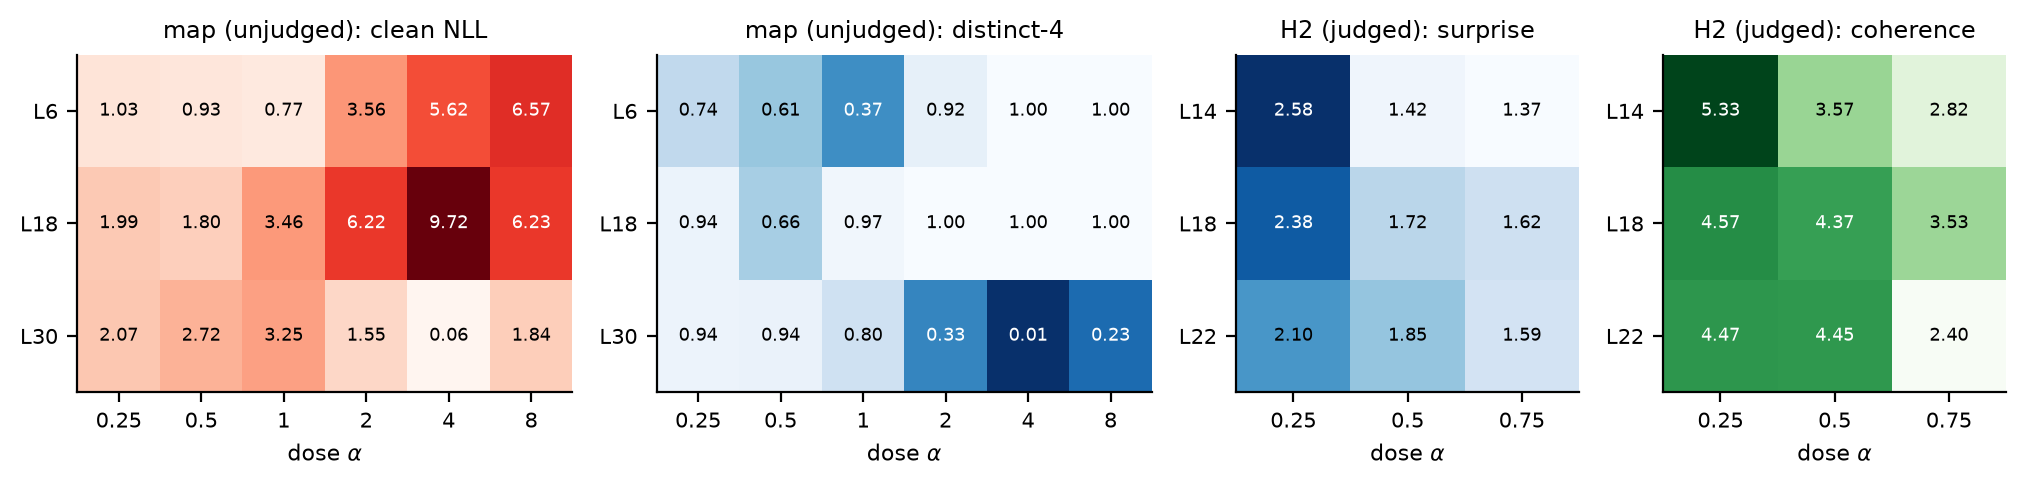
\includegraphics[width=0.98\linewidth]{fig_p4_bandmap.png}
\caption{\textbf{Depth $\times$ dose.} Left pair: the exploratory
57-cell map (layers 6/18/30, continuous translation at doses
0.25--8, three premises each, no judge): clean NLL under the untouched
model and distinct-4: early-layer injection collapses into
low-entropy register basins, late-layer injection at high dose loops
the concept's own token fragment. Right pair: the judged confirmatory
grid (layers 14/18/22, doses 0.25--0.75, ten premises each): surprise
and coherence, both falling with dose at every depth.}
\label{fig:bandmap}
\end{figure}

\begin{figure}[t]
\centering
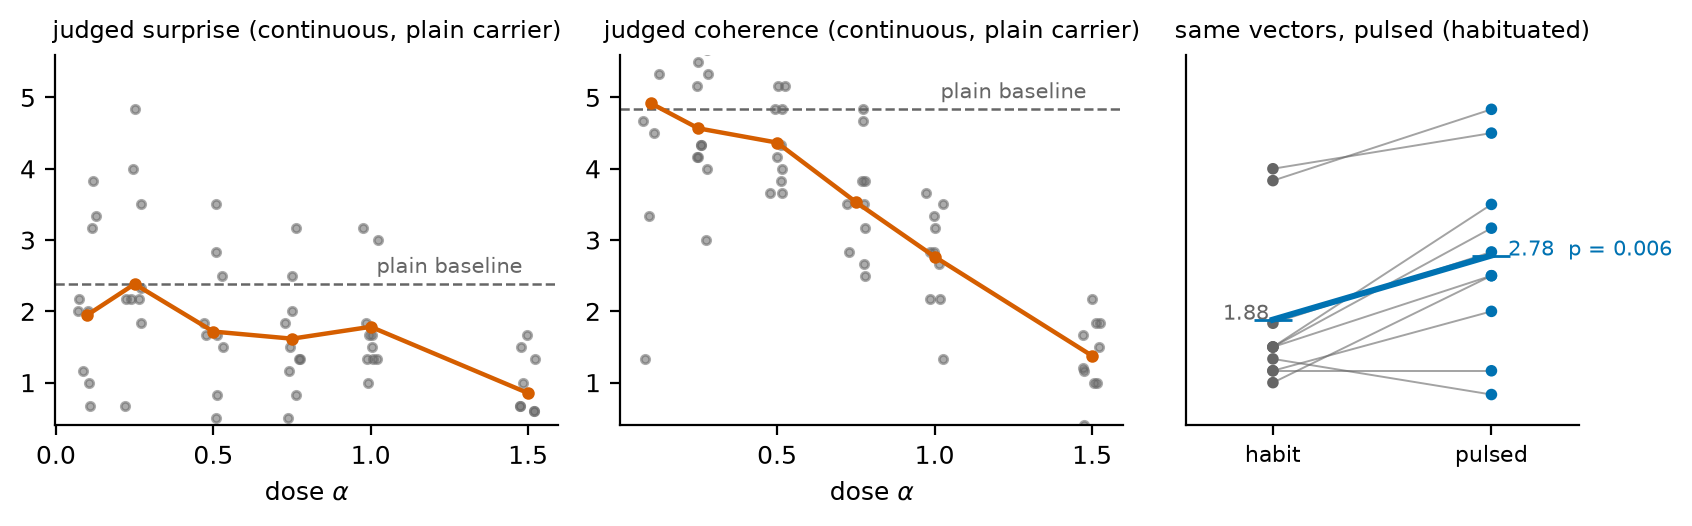
\includegraphics[width=0.98\linewidth]{fig_p4_templaw.png}
\caption{\textbf{The temporal contrast.} Left, center: judged surprise
and coherence at layer 18 as continuous dose rises on the plain
carrier, against that battery's baseline (dashed): more push, less
surprise, collapsing coherence. Right: the four subject directions delivered as
32-token pulses every 300 on the habituated carrier, against that
carrier's own baseline ($+0.90$, $p=0.006$). Points are premise means;
right, error bars are bootstrap 95\% CIs of each mean over premises. The
two panels differ in carrier as well as schedule (see the one-carrier
test in the text).}
\label{fig:templaw}
\end{figure}

\section{Guards change what a dose does; what the pulse buys against the written word}
\label{sec:parity}

The unguarded pulse at dose 1.0 pays in coherence ($-1.01$
\ci{-1.85}{-0.23} against text interruption, two-sided $p=0.049$)
while trailing it in surprise ($-0.86$ \ci{-1.76}{+0.02},
$p=0.10$). The pre-registered guard test
shows the guards do \emph{not} repair this: at equal dose, anchor +
norm shell change coherence by $+0.02$ \ci{-0.65}{+0.63} ($p=0.50$)
while weakening the effective push (clean NLL $2.53 \to 1.83$). Under guards the
ladder $\alpha = 1.0 \to 1.5 \to 2.0$ climbs monotonically in judged
surprise ($2.10 \to 3.23 \to 3.40$) at roughly constant coherence
(Fig.~\ref{fig:ladder}). Because the guards act after the operator,
the nominal dose overstates the displacement they leave behind; the
extension battery therefore logged the \emph{effective} displacement
per burst position, the cosine between the pre- and post-operator
state and the relative norm of the change (Table~\ref{tab:disp}). The
guarded pulse at dose 2.0 leaves the same mean displacement magnitude
as the unguarded pulse at dose 1.0 ($\lVert\Delta h\rVert/\lVert
h\rVert$ $0.75$ in both, with different effective directions by
construction) and a larger surprise gain ($+1.04$ against $+0.40$ over
the carrier; paired over the ten premises, guarded minus unguarded
$+0.64$ \ci{-0.10}{+1.38}, exact two-sided $p=0.094$, a difference
the ten premises do not resolve); the unguarded pulse at 2.0 displaces
twice as much ($1.53$) for less ($+0.86$). So the guards do not
``license dose'' in the sense of admitting a larger push; they change
the composition of the same push (off the premise coordinate, on the
norm shell), and that composition is associated with the larger gain.

\begin{table}[t]
\centering\small
\resizebox{\linewidth}{!}{%
\begin{tabular}{lccccc}
\toprule
arm & $\alpha$ & guards & $\cos(h_{\rm pre},h_{\rm post})$ & $\lVert\Delta h\rVert/\lVert h\rVert$ & $\Delta$ surprise vs carrier \\
\midrule
pulse & 1.0 & none & $0.81$ & $0.75$ & $+0.40$ ($p=0.13$) \\
pulse & 1.5 & none & $0.69$ & $1.13$ & $+0.48$ ($p=0.035$) \\
pulse & 2.0 & none & $0.59$ & $1.53$ & $+0.86$ ($p=0.043$) \\
pulse & 2.0 & anchor + norm shell & $0.72$ & $0.75$ & $+1.04$ ($p=0.012$) \\
sham, random direction & 2.0 & anchor + norm shell & $0.56$ & $0.94$ & $+0.39$ ($p=0.19$) \\
sham, shuffled direction & 2.0 & anchor + norm shell & $0.56$ & $0.94$ & $-0.09$ ($p=0.81$) \\
continuous & 1.0 & none & $0.81$ & $0.77$ & $+0.07$ ($p=0.91$) \\
continuous & 0.107 & none & $1.00$ & $0.08$ & $+0.13$ ($p=0.67$) \\
\bottomrule
\end{tabular}}
\caption{\textbf{Effective displacement and its yield.} Means over
fired positions and ten premises (extension battery, PyTorch bf16);
surprise contrasts paired against the habituated carrier, exact
two-sided sign-flip.}
\label{tab:disp}
\end{table}

At the top of that ladder sits the pre-registered comparison against
the program's flagship prompt-side intervention. Guarded pulse at
dose 2.0 versus text interruption on the ten premises: surprise $3.40$
vs $3.64$ ($\Delta = -0.24$, 95\% $t$ interval \ci{-1.11}{+0.62},
two-sided $p=0.53$),
connection $2.38$ vs $2.39$, coherence within the pre-registered
guard. A non-significant difference is not evidence of equivalence,
and the paired standard deviation here ($1.21$) makes ten premises far
too few to show it: the 90\% confidence interval, \ci{-0.94}{+0.46},
does not fit inside any margin narrower than $\pm 0.95$. The
pre-registered extension therefore reran the trio (habituated
baseline, guarded pulse, text interruption) on thirty premises on
one backend, with an equivalence margin of $\pm 0.75$ fixed in advance
(two one-sided tests; $\pm 0.5$ reported as well). The margin is
$7.5\%$ of the 0--10 scale, about 60\% of text interruption's own effect
over the carrier ($+1.22$), and about one unit of judge noise per
verdict (the original study's test--retest spread); the reader should
note that it admits a deficit of up to $0.7$. On the thirty
premises the difference is $-0.29$ \ci{-0.73}{+0.17} (two-sided
$p=0.23$), the 90\% interval \ci{-0.68}{+0.11} lies inside the
pre-registered band (TOST $p=0.028$; power to show $\pm0.75$
equivalence at the observed paired SD of $1.27$: $0.87$) and not inside
$\pm0.5$ ($p=0.18$); removing self-copied windows changes nothing
($-0.29$, TOST $p=0.029$). Both interventions replicate against the
carrier on the same thirty premises (pulse $+0.93$ \ci{+0.49}{+1.36},
$p=0.0002$; text $+1.22$ \ci{+0.80}{+1.65}, $p<0.0001$), and the
surprise contrast reproduces across backends on the original ten
premises (MLX 8-bit $-0.24$, PyTorch bf16 $-0.29$). That primary, however, is favored by the window layout, and three
things must be said about it before it is read. First, its coherence
guard fails: the median paired coherence change of the pulse against
text is $-1.02$ (mean $-0.90$ \ci{-1.20}{-0.57}, $p<0.0001$), just
beyond the $-1.0$ the paper set for every primary, so by our own rule
the cell-average equivalence carries a failed guard. Second, its power
of $0.87$ is computed at a true difference of zero; at the observed
$-0.29$ it is about $0.61$. Third, the judged windows of the two
arms do not sit at the same distance from the intervention
(\S\ref{sec:instrument}): two of the six grid windows of a state cell
begin at the burst's end, the pulse's best offset, and the original
text arm had no window there. We therefore judged the arms at the same
offsets. Re-judging the state arm and the carrier at $+32$ and $+160$
after each burst end (420 windows, registered after the third round of
AI review) gives a deficit of $-0.34$ \ci{-0.89}{+0.20} (two-sided
$p=0.21$; TOST $\pm0.75$ $p=0.069$, $\pm0.5$ $p=0.28$); and judging
the text arm at $+0$, the window that begins at the end of its injected
sentence (120 windows, registered after the fifth round of AI review; the sentence
sits in the judge's context, never in the graded window), gives text
$5.25$ there against the pulse's $4.03$ at the burst's end
($+1.21$ \ci{+0.75}{+1.67}, two-sided $p<0.0001$; connection $+0.90$,
coherence $+1.38$ in text's favour). With all three
offsets judged in both arms, the fully matched contrast is $-0.73$
\ci{-1.19}{-0.27} (two-sided $p=0.003$; TOST $\pm0.75$
$p=0.46$, $\pm0.5$ $p=0.84$; paired SD $1.23$), and
equivalence is not established. Cell means pool the windows, so the
offsets weigh differently in the two arms (four text windows at $+0$
against the pulse's two burst-end grid windows); weighting the three
offsets equally gives $-0.63$ \ci{-1.09}{-0.16} (two-sided $p=0.01$;
TOST $\pm0.75$ $p=0.29$), so equivalence is not established either
way. The pulse's gain over the carrier at the matched $+32$/$+160$
offsets is intact ($+0.95$ \ci{+0.41}{+1.49}, $p=0.0006$; about $+1.0$
with the burst-end windows included).
The offset curve (Table~\ref{tab:decay}, Fig.~\ref{fig:decay}) shows
the shape: relative to the carrier at the same position, the pulse's
gain is $+1.20$ at the burst's end, $+0.99$ at $+32$ and $+0.90$ at
$+160$; text's is $+1.38$ at $+32$ and $+1.17$ at $+160$; the two raw
curves fall by similar amounts between $+32$ and $+160$ (two points per
arm, no uncertainty attached to the slope), and the pulse sits below at
every offset. What is short-lived is the cost, not the gain: the
pulse's coherence deficit against the carrier is $-1.40$ at the burst's
end, $-1.05$ at $+32$, $-0.82$ at $+160$ and $-0.64$ at $+150$ after
the end (the last grid window), while text's coherence never falls
below the carrier's: the cost halves within a period and does not
vanish. A per-premise regression of the surprise deficit on the
coherence deficit (pulse minus text, 30 pairs) has slope $-0.52$
($p=0.047$): premises where the pulse kept more coherence lost more
surprise, and at equal coherence the fitted deficit is $-0.75$,
descriptive, but a sign that some of the pulse's surprise is bought
with coherence. The other two dimensions do not tie: the pulse trails
text interruption in connection ($-0.52$ \ci{-0.96}{-0.09}, $p=0.03$)
and in coherence ($-0.90$ \ci{-1.20}{-0.57}, $p<0.0001$); the
``identical connection'' of the ten-premise battery did not survive the
extension. The claim, then, is one sentence: a subject placed into the
model's stream as pure activation (harder to read off the text than
a written one, spending no tokens, continuously dosable) raises
judged surprise over the carrier by $+1.0$ where the written subject
raises it by $+1.7$ (averaged over the same three offsets) and sits
below the text at every one of them, at a measurable cost
in how connected and how coherent the resulting text reads. What it is
not: parity, superiority, or evidence that the state reaches value no
prompt reaches (\S\ref{sec:discussion}).

\begin{table}[t]
\centering\small
\resizebox{\linewidth}{!}{%
\begin{tabular}{lcccc|cc|cccc}
\toprule
 & \multicolumn{4}{c|}{judged surprise} & \multicolumn{2}{c|}{connection} & \multicolumn{4}{c}{coherence} \\
arm & burst end & $+32$ & $+160$ & $+150$ & $+32$ & $+160$ & burst end & $+32$ & $+160$ & $+150$ \\
\midrule
text interruption & $5.25$ & $4.09$ & $3.67$ & n/a & $2.71$ & $2.91$ & $4.85$ & $4.97$ & $4.89$ & n/a \\
guarded pulse, $\alpha{=}2.0$ & $4.03$ & $3.70$ & $3.40$ & $3.42$ & $2.24$ & $2.23$ & $3.47$ & $3.57$ & $4.02$ & $4.33$ \\
habituated carrier & $2.83$ & $2.71$ & $2.50$ & $2.62$ & $2.04$ & $1.94$ & $4.87$ & $4.62$ & $4.84$ & $4.97$ \\
\bottomrule
\end{tabular}}
\caption{\textbf{Decay by offset from the intervention.} Mean judged
scores over thirty premises at windows beginning at the stated offset
after the end of the injected sentence (text) or of the burst (pulse;
the carrier at the same positions). The $+32$/$+160$ state windows are
the matched re-judging (after AI review round 3) and the text arm's ``burst end''
column is the $+0$ re-judging (after AI review round 5); the state arms' ``burst end''
and $+150$ (the grid window that begins 182 tokens after the burst's
start, i.e.\ 150 after its end) come from the original grid. Connection
at $+0$ for text: $3.24$ (pulse $2.34$).}
\label{tab:decay}
\end{table}

\begin{figure}[t]
\centering
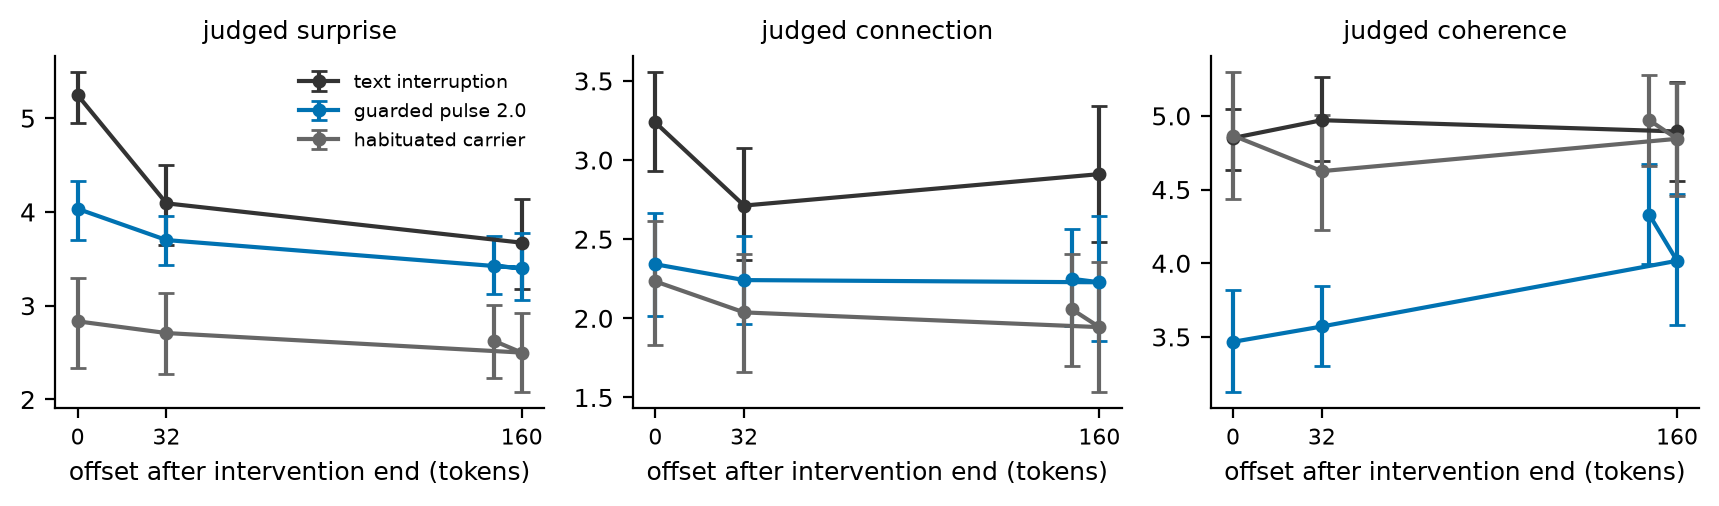
\includegraphics[width=0.98\linewidth]{fig_p4_decay.png}
\caption{\textbf{Decay by offset.} The three judged dimensions against
the offset after the intervention end, thirty premises, bootstrap 95\%
CIs of the mean over premises. Surprise: the pulse sits below the text at every matched offset,
including the burst's end once the text arm is judged there ($+0$).
The pulse and the carrier carry one further grid point, 150 tokens
after the burst's end. Coherence: the pulse's cost is front-loaded and
halves within the period.}
\label{fig:decay}
\end{figure}

\paragraph{Does the content of the pulse matter?} A pulse could work
by carrying a subject or merely by perturbing a habituated orbit. Two
pre-registered shams keep everything about the guarded pulse (dose
2.0, schedule, guards, rotation) and replace the direction: a random
unit vector per subject, and the subject's own direction with its
coordinates shuffled (same norm and entry distribution, no meaning in
the model's basis). Both shams displace the state \emph{more} than the
real pulse (Table~\ref{tab:disp}) and yield less: the real pulse
beats the random-direction sham by $+0.65$ \ci{+0.13}{+1.18}
(one-sided $p=0.029$, BH $q=0.07$, short of the family threshold)
and the shuffled-direction sham by $+1.13$ \ci{+0.65}{+1.65}
($p=0.001$, $q=0.005$); against the carrier the shams themselves move
$+0.39$ ($p=0.19$) and $-0.09$ ($p=0.81$).
The shams are not less coherent than the real pulse (coherence $+0.23$
\ci{-0.38}{+0.84} and $+0.36$ \ci{-0.28}{+1.01} relative to it), so the
judge is not marking them down for damage. The clean result is the
shuffled sham, which keeps the direction's norm and coordinate
statistics and loses only its meaning; the random-direction sham is
consistent with it. A meaningful direction, not the perturbation of an
orbit, carries the effect. Both shams lie outside the set of directions
the model itself uses, so they separate meaning from noise; whether
\emph{this} subject's direction does more than another semantic
direction would (a fifth subject, another premise's direction) is not
tested here, and a semantic sham matched in displacement is registered
as future work. A blind manipulation check completes the picture: for
the four windows per cell that begin at the end of each burst or
injection (positions $300k{+}32$; the surprise judge graded two of these
per state cell), a separate judge call ($k{=}1$) names which of the
four subjects, if any, the window engages, with the options shuffled
per window; text interruption is the positive control and the
habituated carrier gives the base rate (Table~\ref{tab:manip}). Two
nulls are reported: among the windows where the judge names a subject,
chance is 25\%; over all windows, a conservative null treats every
window as a guess at 25\%. The subject reaches the judged text in about
half of the text-interruption windows (49\% of windows; 19 of 25 picks
correct, binomial $p=10^{-7}$ among picks, $p=0.001$ over windows) and
in about a quarter of the guarded-pulse windows at dose 2.0 (23\%; 9
of 14 picks, $p=0.002$ among picks, not significant over windows),
against zero correct picks on the carrier (6 spurious picks in 40
windows); the weak state arms (unguarded pulse, guarded pulse at
dose 1.0, repulsion, rotor) transfer nothing detectable (2--8\%).
Content transfer by the pulse is therefore detectable (significant
among picks on the MLX parity battery), dose-dependent under guards, and
about half as frequent as by text. In the extension battery, on the
other backend, the rates are text 34\%, guarded pulse 14\% (17 of 53
picks correct, $p=0.15$ among picks: not significant on this backend),
reset interruption 18\%, continuous injection at $\alpha=1.0$ 44\% (the
subject arrives, in degenerate prose) and the two shams 3--5\%, the
carrier's base rate; the full counts and both nulls are in the
manipulation-check appendix. The pulse's judged surprise sits below
text interruption's while it places its subject in the text less often;
the shams show that what it does place there is what matters.

\begin{table}[t]
\centering\small
\resizebox{0.98\linewidth}{!}{%
\begin{tabular}{lcccc}
\toprule
arm & windows & subject named correctly & of windows with a pick & ``none'' \\
\midrule
habituated carrier (base rate) & 40 & no subject & 0/6 & 85\% \\
text interruption & 39 & 49\% \ci{34}{64} & 19/25 & 36\% \\
guarded pulse, $\alpha{=}2.0$ & 39 & 23\% \ci{13}{38} & 9/14 & 64\% \\
guarded pulse, $\alpha{=}1.5$ & 40 & 25\% \ci{14}{40} & 10/21 & 48\% \\
guarded pulse, $\alpha{=}1.0$ & 40 & 5\% \ci{1}{17} & 2/5 & 88\% \\
unguarded pulse, $\alpha{=}1.0$ & 39 & 8\% \ci{3}{20} & 3/7 & 82\% \\
repulsion (anchored / not) & 40 / 40 & 2\% / 5\% & 1/4, 2/8 & 90\% / 80\% \\
rotor & 39 & 3\% \ci{0}{13} & 1/4 & 90\% \\
\bottomrule
\end{tabular}}
\caption{\textbf{Manipulation check} (parity battery, MLX). A blind
judge ($k{=}1$) names the subject active at each burst-end window;
``subject named correctly'' is over all windows (Wilson 95\% CIs), ``of
windows with a pick'' gives correct/picks, whose null is 25\%.}
\label{tab:manip}
\end{table}

\paragraph{The comparator.} Text interruption in the preserved context
is the strongest prompt-side intervention of the original study
\emph{among those that keep the context}; its reset variant (the
context replaced by the premise and the new subject at every period)
scored as well or better in coherence there. The pre-registered
extension includes that reset comparator on the ten premises, and it
is the strongest arm of the battery: $+1.62$ over the carrier in
surprise with the highest coherence ($5.13$). The guarded pulse trails
it by $-0.58$ \ci{-0.99}{-0.09} (two-sided $p=0.043$, BH $q=0.07$)
with the coherence guard failing ($-1.01$). Against the strongest
prompt-side intervention we know, then, the state channel is not at
parity: it trails the preserved-context interruption at matched offsets
(equivalent within $\pm0.75$ only on the cell average) and trails the
reset one.

Two declared secondaries returned honest negatives. A first-version
rotor (rotating the premise--subject plane, $\theta=0.8$) underperforms
text interruption ($-1.53$ \ci{-2.43}{-0.63}, $p=0.014$, BH
$q=0.055$; a later cheap screen located its useful range at $\theta
\in [1.2, 1.6]$, an untuned operator, not a dead one). And the
program's own registered prediction failed: pulsed state repulsion
\emph{without} an anchor did not degenerate (anchored minus
unanchored coherence $-0.53$ \ci{-1.18}{+0.02}, the wrong sign for the
prediction), refusing the fourth appearance of the anchor law (the
program's finding, in weights and in behavior, that repulsion without a
fixed reference degenerates); a stress screen then showed why:
repulsion from a \emph{moving} mean is self-limiting, because the
reference chases the state. The anchor law, as established in weights
and behavior, is about fixed references.

\begin{figure}[t]
\centering
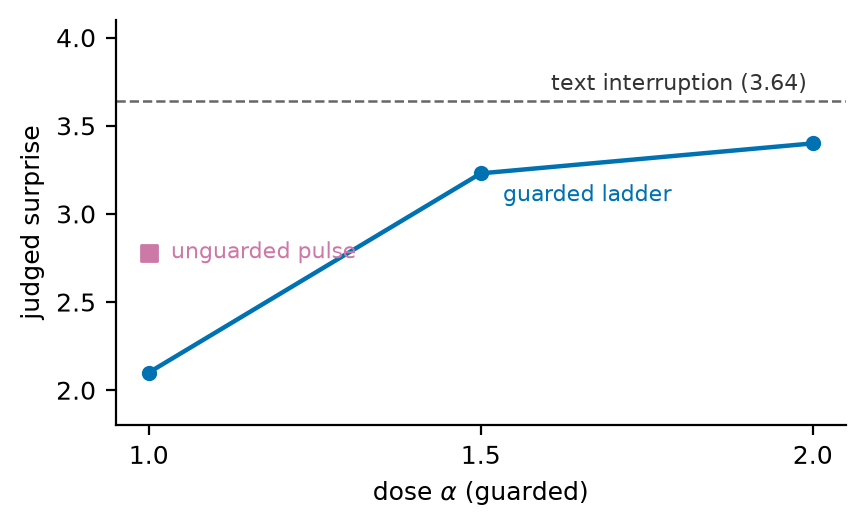
\includegraphics[width=0.72\linewidth]{fig_p4_ladder.png}
\caption{\textbf{Guards change what a dose does.} Judged surprise of the guarded
pulse at doses 1.0/1.5/2.0 (points), with the unguarded pulse (square)
and the text-interruption reference (dashed line), ten premises each.
The ladder reaches the reference within the resolution of ten
premises; the equivalence test is in the text.}
\label{fig:ladder}
\end{figure}

\section{Generality: the pattern travels in-family}
\label{sec:generality}

The pre-registered generality battery reran the decisive trio
(habituated baseline, guarded pulse at dose 2.0, text interruption)
on three untouched models, with the layer at 50\% of each network's
depth and the dose carried over unchanged in premise-norm units (a
convention, not a calibration).

\textbf{Qwen3-14B-Base (Hugging Face id \texttt{Qwen/Qwen3-14B-Base};
same family, larger): the primary replicates.} Pulse
over habituation $+1.083$ \ci{+0.567}{+1.617}, $p=0.0020$, coherence
guard clean; against text interruption, a tie of the means at $n=10$
(on the cell-average window layout, which \S\ref{sec:parity} shows
favours the pulse; the 14B cells were not re-judged at matched offsets):
surprise $3.48$ vs $3.48$ ($p=0.99$; indistinguishable at this sample
size, not equivalent). The dimensionless dose and proportional-depth
layer worked without retuning on this model.

\textbf{Qwen3.8-27B (Hugging Face id \texttt{Qwen/Qwen3.8-27B}; a
later generation than the Qwen3-8B origin model, aligned): the carrier
breaks, not the phenomenon.} Under our base-model protocol, which bans EOS
and forces 1500 tokens, this chat-trained model opens with fluent
prose and collapses into token salad past its natural turn end
(judge notes: ``degenerate token soup''). A nominally significant
pulse effect inside that salad ($p=0.041$) does not count as support,
and we do not count it. Aligned carriers need their own protocol
(chat-formatted seeding, free EOS, natural lengths); this is future
work, not a footnote.

\textbf{OLMo-2-13B (different family): no reading.} Pulse minus
habituation $-0.09$ ($p=0.78$). All three arms, however, sit in an
encyclopedic register basin (judged coherence $0.4$--$0.6$ everywhere),
the OLMo analogue of the register basins of \S\ref{sec:temporal}, and
the judge's refusals on this model are not uniform across arms: of the
scheduled windows, 12\% (habituated), 14\% (interrupted) and 28\%
(pulsed) were dropped because every call refused or returned unparsable
verdicts, and the surviving windows average 4.4, 4.0 and 4.7 calls
rather than 5. Refusals are selective for degenerate text, so the
surviving subset is selected differently per arm, most heavily in the
pulsed arm; the OLMo contrast is therefore reported without a reading,
like the 27B's. On Qwen3.8-27B the drops were 25/23/22\% and on the
origin model negligible (6 refused calls in the parity battery). A
fourth rung registered in the same battery, gpt-oss-120b, was attempted
and abandoned before any cell was judged (mxfp4 kernel failures on the
rented GPU). Whether an OLMo null would reflect family-dependence of
the phenomenon or miscalibration of layer and dose for this family
cannot be separated here; per-model calibration and a
degeneration-tolerant judge prompt are registered future work. The
generality claim we make is therefore exactly this: \emph{the pattern
replicates across scale within a family; family-generality is open}.

\begin{table}[t]
\centering\small
\resizebox{\linewidth}{!}{%
\begin{tabular}{lccc}
\toprule
model & pulse $-$ habit (primary) & pulse $-$ inter & verdict \\
\midrule
Qwen3-8B-Base (origin, 10 premises, MLX) & $+0.90$ \ci{+0.45}{+1.33}, $p=0.006$ & $-0.24$ \ci{-1.11}{+0.62}$^{t}$, $p=0.53$ & indistinguishable \\
Qwen3-8B-Base (30 premises, PyTorch) & $+0.93$ \ci{+0.49}{+1.36}, $p=0.0002$ & $-0.29$ \ci{-0.73}{+0.17}, $p=0.23$ (cell average); $-0.73$ \ci{-1.19}{-0.27}$^{t}$, $p=0.003$ (matched) & below text \\
Qwen3-14B-Base & $+1.08$ \ci{+0.57}{+1.62}, $p=0.002$ & $+0.00$ \ci{-0.44}{+0.43}, $p=0.99$ & tie of means \\
Qwen3.8-27B (aligned) & $+0.20$ \ci{+0.02}{+0.38}, $p=0.041$ & $+0.14$ \ci{-0.03}{+0.31}, $p=0.16$ & no reading (carrier breaks) \\
OLMo-2-13B & $-0.09$ \ci{-0.32}{+0.11}, $p=0.78$ & $-0.09$ \ci{-0.37}{+0.11}, $p=0.68$ & no reading (register basin; refusals not uniform; text $-0.00$ too) \\
\bottomrule
\end{tabular}}
\caption{\textbf{The generality ladder.} Judged-surprise contrasts,
paired over the ten premises (thirty in the second row); doses in
premise-norm units and layers at 50\% depth, carried over by convention
without retuning. ``Tie'' means indistinguishable at $n=10$, not
equivalence. Intervals are percentile bootstraps except those marked $t$
(95\% $t$ intervals; for the first row's, the percentile interval,
\ci{-0.94}{+0.47}, matches a 90\% $t$ interval).}
\label{tab:ladder}
\end{table}

\section{Spectra: orbits, sentence rhythm, and what flattening survives}
\label{sec:mechanism}

Why does the pulse work where pressure fails? A measurement study
replayed finished cells through the model, capturing the mid-layer
trajectory, and compared the state autocorrelation
$A_{\mathrm{state}}(\tau)$ (unit-normed, mean-centered states) against
the token autocorrelation (the ground truth of literal loops), reading
the strongest detrended local peak of each ($\tau \ge 5$; literal
period-2 loops sit below the reader's floor and are noted as a blind
spot).

The prominence ladder in the illustrative cells is clean
(Fig.~\ref{fig:spectra}). A literal phrase loop shows a state period
matching the phrase length ($P=7$, prominence $0.44$). Register
collapses (the quiz mode, the math-exercise mode) show matched
token--state periodicity at their block rhythms ($P=123$ and $84$). And
a habituated cell that repeats no phrase still shows matched
token--state periodicity at $P\approx 30$ (prominence $0.18/0.15$),
whose text reads as sentence-level cycling through the same cast,
the ``return to the theme, not the sentence'' of
\citet{ono2026interrupting}.

Those are single cells, and the population reading is more modest.
Replaying every cell of the parity battery (90 cells, 9
arms, 10 premises each) and adding the null a state period has to beat
(the autocorrelation of the sentence-boundary indicator, i.e.\ the
rhythm of sentences) gives Table~\ref{tab:spectra}. Sentence rhythm
is the dominant periodicity in every arm (punctuation prominence
$0.10$--$0.17$); the state prominence of the habituated carrier is
small ($0.039$ \ci{0.016}{0.070}) and its period coincides with the
punctuation period in 4 of 10 cells, including the $P{=}30$ cell
above, whose punctuation period is also 30. What survives as an
orbit-flattening effect is specific: the guarded pulse at dose 2.0
lowers state prominence against the paired carrier by $-0.029$
\ci{-0.057}{-0.008} (exact two-sided $p=0.006$), and at dose 1.5 by
$-0.027$ ($p=0.02$); text interruption trends the same way ($-0.023$,
$p=0.22$); the unguarded pulse, the rotor and moving-mean repulsion do
not flatten anything. One more caution: the punctuation prominence
also falls in the winning arm ($0.095$ against $0.132$), and per-premise
changes in state and punctuation prominence correlate ($r \approx 0.6$),
so part of the state flattening is the sentence rhythm flattening.
Masking the punctuation period ($\pm20\%$) leaves a residual state
flattening for the guarded pulse at 2.0 (mean $-0.023$; exact sign-flip
$p=0.010$, i.e.\ nearly every premise moves the same way, while the 95\%
$t$ interval \ci{-0.048}{+0.002} touches zero because two premises
carry most of the magnitude) and at 1.5 ($p=0.02$), not for
interruption ($p=0.08$); the per-arm paired contrasts, the masked
residuals and the state--punctuation correlations are tabulated in the
released spectral appendix. This section is descriptive, and the exact
test is the statement we make. We therefore retract the general form of the claim: the
interventions a judge rewards are not all spectral flatteners, and the
habituated ``silent orbit'' is largely the rhythm of sentences. The
specific form (the winning state arm carries the flattest trajectory
in the battery, part of which survives the sentence-rhythm null) is
descriptive, not causal.

\begin{table}[t]
\centering\small
\resizebox{\linewidth}{!}{%
\begin{tabular}{lcccc}
\toprule
arm & state prominence [CI] & $\Delta$ vs habit ($p$) & punct.\ prominence & $P_{\rm state}{=}P_{\rm punct}$ \\
\midrule
habit & $0.039$ \ci{0.016}{0.070} & n/a & $0.132$ & 4/10 \\
inter & $0.016$ \ci{0.009}{0.026} & $-0.023$ ($0.22$) & $0.118$ & 3/10 \\
pulse ($\alpha{=}1$) & $0.035$ \ci{0.010}{0.080} & $-0.004$ ($0.77$) & $0.137$ & 4/10 \\
pulseG ($\alpha{=}1$) & $0.054$ \ci{0.016}{0.113} & $+0.014$ ($0.57$) & $0.157$ & 1/10 \\
pulseG ($\alpha{=}1.5$) & $0.013$ \ci{0.008}{0.018} & $-0.027$ ($0.02$) & $0.100$ & 3/10 \\
pulseG ($\alpha{=}2$) & $0.010$ \ci{0.007}{0.015} & $-0.029$ ($0.006$) & $0.095$ & 3/10 \\
repelA & $0.022$ \ci{0.012}{0.038} & $-0.018$ ($0.12$) & $0.113$ & 4/10 \\
repelN & $0.028$ \ci{0.010}{0.050} & $-0.012$ ($0.64$) & $0.115$ & 1/10 \\
rotor & $0.078$ \ci{0.013}{0.181} & $+0.039$ ($0.91$) & $0.169$ & 3/10 \\
\bottomrule
\end{tabular}}
\caption{\textbf{Spectra of the whole battery.} Dominant detrended
local peak of the state autocorrelation per cell; bootstrap CIs over
the ten premises; paired differences against the habituated carrier
with exact sign-flip $p$; the sentence-boundary autocorrelation as the
rhythm null; and how often the state period equals the punctuation
period within 20\%.}
\label{tab:spectra}
\end{table}

\begin{figure}[t]
\centering
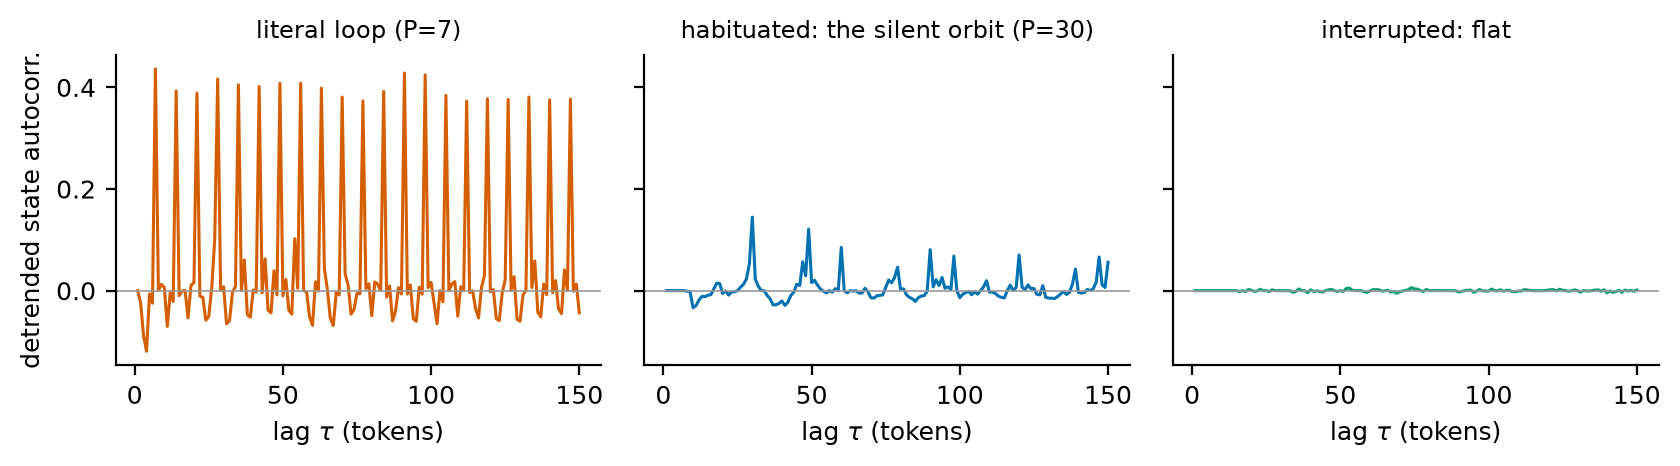
\includegraphics[width=0.98\linewidth]{fig_p4_spectra.png}
\caption{\textbf{Silent orbits and their removal: three illustrative
single cells.} Detrended state autocorrelation for a literal loop
(state period = phrase length), a habituated cell (the silent orbit at
$P\approx30$, matched in tokens and matched by the punctuation
period, see the text), and an interrupted cell (flat). The population
contrast for interruption is not significant (Table~\ref{tab:spectra});
the arm that flattens at the population level is the guarded pulse.}
\label{fig:spectra}
\end{figure}

\section{The verified null, and its floor}
\label{sec:verified}

Do these operators buy anything a verifier can price? The
pre-registered battery ran three arms, untouched carrier, pulses
toward narrative subjects (the cross-register wildcard) and pulses
toward the domain's own thinking prompts, with the same configuration as
the parity battery (Qwen3-8B-Base on MLX, layer 18, guarded pulse at
dose 2.0 with anchor and norm shell, bursts of 32 every 300 tokens, the
four narrative directions of \S\ref{sec:instrument}) inside verified
bin-packing notebook generation (16 distribution variants including the far family
of \citet{ono2026mass}, 6 notebooks each, 288 notebooks), scoring with
the exact evaluator against best-fit and first-fit.

The pre-registered primary is null: per-variant best distance to the
classics, wildcard minus control $+0.00014$ \ci{+0.00000}{+0.00036},
one-sided $p=1.0$; transfer and far-family contrasts null; the single
best gap across all three arms identical to five decimals ($-0.00334$).
The full ledger explains the identity (Table~\ref{tab:bconf}): the
untouched carrier had already matched the classics in \textbf{16 of 16}
variants (reproducing best-fit gives a gap of exactly zero), so the
pre-registered measure was saturated by a trivial strategy in every
cell; programs that beat the classics do occur (two, one and three
finds per arm), but at six notebooks per variant the battery has no
power on find rates. The battery therefore does not support a
dissociation between judged experience and verified value; it shows
that the verified task, at this scale, offers no headroom for any
intervention to be measured on. What the ledger does show is a cost:
the wildcard arm produced fewer valid programs (121 against 165 for the
carrier; paired over the sixteen variants, $-2.75$ valid programs per
variant \ci{-4.69}{-0.75}, exact two-sided $p=0.023$, lower in 11 of
16) at the same best value. (An earlier 120-notebook
screen had produced a lone wildcard find; the confirmatory dissolved it
into sampling noise: all arms find occasionally at $n{=}6$.) A
first-version route-blocking operator (projecting out the top
principal directions of a previous solution's trajectory) behaved as
a mild handicap: production down, no depth gained, and a calibration
curve showing that the top trajectory components carry the
code-writing machinery itself (blocking $\ge 4$ directions removes the
faculty, not the idea).

\begin{table}[t]
\centering\small
\begin{tabular}{lcccccc}
\toprule
arm & candidates & valid & distinct & mean gap & best gap & finds \\
\midrule
carrier (none) & 293 & 165 & 165 & $+0.0215$ & $-0.00334$ & 2 \\
wildcard pulse & 278 & 121 & 120 & $+0.0194$ & $-0.00334$ & 1 \\
domain pulse & 308 & 161 & 157 & $+0.0242$ & $-0.00334$ & 3 \\
\bottomrule
\end{tabular}
\caption{\textbf{Verified battery, full ledger.} Gap = train excess
over $\min$(best-fit, first-fit); ``find'' = a program beating both
classics on its variant. Variants with headroom for the carrier: 0 of
16.}
\label{tab:bconf}
\end{table}

Consistent with the attractor results of \citet{ono2026mass}, the
verified value reachable by this carrier behaves as a constant that
state stimulation did not move; whether it \emph{could} move it on a
task with headroom is untested here.

\section{Boundaries}
\label{sec:boundaries}

For designers of state interventions, the mapped edges: (i) \emph{depth
matters more than dose}: early layers destabilize into register
basins, late layers are token bias (at high dose the injected concept's
token fragment loops literally); (ii) \emph{guards change the composition of a push, not its size}; (iii)
\emph{moving-reference repulsion is self-limiting}: collapse
requires a fixed reference, which reframes the anchor law; (iv)
\emph{aligned models are a different carrier}: forced continuation
past the turn end manufactures degeneration that no operator caused;
(v) judged-surprise instruments punish degeneration (they cannot be
gamed by noise), but they refuse some degenerate text outright, which
costs coverage and must be reported.

\section{Related work}
\label{sec:related}

\paragraph{Activation steering: what is injected, when, and how it is
judged.} Adding a vector to the residual stream during generation has a
decade of ancestry. PPLM perturbed activations toward a topic during
open-ended generation and measured whether the topic reached the text
and at what cost in fluency \citep{dathathri2020pplm}, the direct
ancestor of our manipulation check; latent steering vectors were
extracted from a pretrained model and added to its hidden states to
reproduce target sentences \citep{subramani2022latent}; and in-context
vectors replace textual demonstrations with a latent shift applied
during generation \citep{liu2023icv}, the closest precedent to our
question of state against written word, though without a prompt-matched
rival. The recent additive family (ActAdd \citep{turner2023actadd},
contrastive activation addition \citep{panickssery2023caa}, truthfulness
intervention \citep{li2023iti}, representation engineering
\citep{zou2023repe}, SAE features \citep{cunningham2023sae,templeton2024scaling},
function vectors \citep{todd2023function} and refusal-direction ablation
\citep{arditi2024refusal}) steers style, safety and factual behavior,
and alignment training itself has been read as learning to steer around
such directions \citep{lee2024mechanistic}. Refinements of the additive
vector anticipate elements of our instrument: mean-centring corrects the
direction for the dataset's offset \citep{jorgensen2023mean};
Householder pseudo-rotation edits direction while preserving magnitude
\citep{pham2024householder}, the norm-preserving intent our norm shell
shares; conceptors replace the additive vector by soft projections onto
an ellipsoid, with Boolean combinations \citep{postmus2024conceptors},
which is where our projection operator should be placed; and conditional
activation steering \citep{lee2025programming} gates the edit on a
condition, a \emph{when} chosen by the input, where our pulse chooses
it by the clock (we know no precedent for clock-scheduled steering, and
claim only that we found none). \citet{tan2024analysing} document how
unreliable steering vectors are across prompts, which is one reason we
report per-premise pairs and effective displacement rather than nominal
dose. On creativity specifically, a steering direction extracted from
``boring'' versus ``creative'' prompting raises rated creativity when
added at inference \citep{olson2024creativity}; Stiefel activation
steering explores multiple orthogonal directions for diverse generation
\citep{zhu2026stars}; and CreativityNeuro reports that weight-space
steering generalises to open creative tasks where activation steering
does not \citep{schapiro2026creativityneuro}, a negative for the
latent channel that is consistent with, and sharper than, the deficit we
measure against the written word. None of these compares the latent
channel with a prompt-matched textual rival under a judge that never
sees the intervention, and that comparison is what this paper adds.
\citet{mishra2026nonsurjective} show, under stated assumptions and
empirically, that steered states are unreachable by prompts but do not
test their value; our result is one value measurement in that space,
and it constrains easy versions of the fertility hypothesis. Weight-space
analogues (task arithmetic \citep{ilharco2022task} and the weight
steering above) edit the persistent model where we perturb the
transient thought.

\paragraph{Repetition and orbits.} The loop we measure as a silent
orbit has a literal ancestor in the repetition problem: its
self-reinforcing dynamics \citep{xu2022learning}, its roots in
training data \citep{li2023repetition}, and dedicated neurons
\citep{hiraoka2025repetition}. Habituation suppresses the literal
form; the state-space rhythm that survives it is what \S\ref{sec:mechanism}
characterizes. Rotations of the residual stream are not exotic to the
architecture (rotary position embeddings \citep{su2024roformer}
rotate query--key pairs by position), but ours act on content
directions, not positions.

\paragraph{Latent computation.} Recurrent-depth and looped transformers
move computation from tokens into the residual stream: a learned router
decides how many times a token passes through shared blocks
\citep{bae2025mor}, or a recurrent block is unrolled at test time to
scale reasoning without emitting text \citep{geiping2025recurrent}. In
such models the question this paper asks of the residual stream,
what an intervention there buys relative to the written word, stops
being a question about steering and becomes one about the model's
primary channel of thought. We note, as speculation rather than a
result, that the property we measure (a state injection is harder
to read off the text than a written one, \S\ref{sec:parity}) would
then bear on monitoring; we measured the transfer of a subject to the
text, not the detectability of the intervention.

\paragraph{Mechanistic intervention.} Causal tracing and model editing
record and modify internal routes to \emph{explain} behavior
\citep{meng2022rome}; our route-blocking screen inverts the direction
, recording a route to \emph{forbid} it, and reports the first
calibration of how much of a trajectory can be blocked before the
faculty, not the idea, is removed.

\paragraph{Decoding-time control.} Degeneration under maximization
\citep{holtzman2020curious} anticipates our salad regimes;
contrastive decoding \citep{li2022contrastive} and proxy tuning
\citep{liu2024proxy} intervene through logits of a second model, a
surface channel our late-layer results effectively reproduce
(late-layer injection $\approx$ token bias); PPLM
\citep{dathathri2020pplm} is the activation-level counterpart of that
family; the mid-network channel studied here is what logit-level
methods cannot reach.

\paragraph{The program.} Protocol, habituation and interruption from
\citet{ono2026interrupting}; consolidation, tails and the attractor
from \citet{ono2026mass}; the operator-package factorial from the
companion verified-search paper \citep{ono2026operator}. The automated-researcher study of
\citet{chen2026automated} independently reports the program's telemetry
(method monocultures, flat idea diversity under climbing scores,
capability anchors) at industrial scale in an alignment-mitigation
setting, a mass regime, complementary to the frontier questions
here.

\section{Discussion and limitations}
\label{sec:discussion}

\paragraph{What the state channel buys.} A new channel into the
model's ongoing thought exists, is dosable and reversible, spends no
context, and is harder to read off the text than a written subject.
What it buys, measured against the written subject it was modeled on:
a gain in judged surprise that sits below the text's at every matched
offset ($-0.73$ on thirty premises with all three offsets judged in both
arms; equivalent within $\pm0.75$ only on the cell average that
contains the pulse's best offset, and there with a failed coherence
guard); carried by a meaningful direction (the shams fail; the
manipulation check finds the subject in the text); and paid for in
connection and in a coherence cost that is front-loaded, halves within
about 150 tokens and does not vanish, with a clear deficit against the
reset interruption. This is the state chapter of a four-substrate
series (token, context, weights, state), and its verdict on the
inference-time fertility hypothesis is the one the abstract states:
latent injection buys a content-specific gain in judged novelty that
stays below the written word's, at a coherence cost, not more than the
written word. The strong hypothesis, that prompt-unreachable states
yield value prompts cannot, remains open; the continuous-injection
null and the deficit of the pulse are its first constraining data
points. The subject reached the judged text in 14--23\% of burst-end
windows when injected as state, against 34--49\% when written; we note
in \S\ref{sec:related} why that might matter for monitoring, as
speculation.

\paragraph{Experience versus value.} We had hoped to report a
dissociation: state operators changing what a judge experiences
while leaving what a verifier prices untouched. The verified battery
cannot carry that claim: its measure had no headroom. What survives is
weaker and still worth stating: on the one verified task we ran, the
operators that a judge cannot tell from the written word produced no
verified gain and fewer valid programs.

\paragraph{Limitations.} The ten confirmatory premises are reused
across this paper's batteries (each analysis pre-registered before its
data, but adaptation risk accumulates and is declared; the equivalence
extension adds twenty premises unused by any earlier battery of this
paper). The judge is a single instrument (one model family; its
test--retest behavior was measured in \citealp{ono2026interrupting});
generality is established across scale, not family; doses and layers
were calibrated on the origin model and carried to others by
convention (50\% depth, premise-norm units) rather than per-model
tuning; the verified domain is one task family and, as reported, had
no headroom. The two backends do not give the same carrier: on the ten
confirmatory premises the habituated 8-bit MLX carrier scores $1.88$ in
surprise against $2.48$ for the bf16 PyTorch carrier, while the
interventions land within $0.1$--$0.2$ of each other across backends
($2.78$/$2.87$ unguarded pulse, $3.40$/$3.52$ guarded, $3.64$/$3.80$
text); contrasts against the carrier are therefore larger under
quantization, and the unguarded pulse at dose 1.0 is significant on one
backend only. The judge was the same model on both, called on different
dates (\S\ref{sec:instrument}), so judge drift and quantization are
confounded in that comparison. Bit-identical operators do not imply
comparable generation across weight precisions. The plain-carrier
dose--response and the habituated pulse differ in carrier, in schedule
and in direction; the one-carrier test of \S\ref{sec:temporal} is the
only clean temporal contrast, and its thirty-premise verdict was
reached under a rule that admitted either of two contrasts and by
extending ten pairs already read with twenty new ones; the contrast
survives on the twenty new pairs alone. The equivalence result holds
for judged surprise only, at the $\pm0.75$ margin only, against the
preserved-context interruption only, on the cell-averaged windows only,
and with its coherence guard failed; at matched offsets it is not
established, and the matched re-judgings were registered after the
third and fifth rounds of review by AI reviewer agents, before judging,
with the primary result known. All text is English narrative prose from opening sentences; the
thirty premises are the ten confirmatory and ten original premises of
\citet{ono2026interrupting} plus ten expository openings from the same
source, and the pulse's deficit against text is largest in the
expository pool ($-0.82$ in surprise; coherence $3.82$ against
$4.87$), so genre is a variable the design does not control. The layer
(18 of 36) and the doses were chosen on the exploratory map of the
origin model and carried to the others by convention; dependence on
that choice is not mapped. Every cell is 1500 tokens; the batteries
ran on one laptop (MLX) and single rented GPUs (PyTorch), with judge
costs of the order of tens of dollars per battery: office scale, not
a sweep. The mechanism (why 32-token pulses raise judged surprise where
constant pressure degrades) is characterized spectrally, not causally.

\paragraph{Future work.} Registered and not run: a duty-cycle sweep
at equal integrated dose (the schedule test proper); a semantic sham
(a fifth subject, or another premise's direction) and a sham matched
in effective displacement; the OLMo trio on a reset carrier and a
degeneration-tolerant judge prompt; a re-judging of a sample of MLX
cells on the PyTorch judge dates. Beyond that: a protocol for aligned
carriers; per-model calibration for cross-family tests; the strong
fertility test on a carrier where the pulse and the word are both at
ceiling; and substrate-level questions (consolidating the search's
schematic memory rather than its winners, and cross-model state
transfer) that the present results motivate but do not touch.

\section*{Reproducibility and provenance}
The operator algebra, both backends and the generation, judging and
analysis scripts are in the code repository
\url{https://github.com/RobertoOno/interrupting-the-loop} as of 10 September
2026; the complete code, including the scripts and appendix sections added
after that date, is in an evidence deposit on Zenodo,
doi:\href{https://doi.org/\evidencedoi}{\evidencedoi}. The cells and judge
verdicts of every battery, including the matched-offset re-judging of
\S\ref{sec:parity}, are in the repository's release \texttt{run-data-v2},
archived as Zenodo
\href{https://doi.org/10.5281/zenodo.22714138}{10.5281/zenodo.22714138};
the $+0$ re-judging, made after that release, the run logs and the dated
pre-registration entries, excerpted from the project notebook (in
Portuguese), are in the evidence deposit. All confirmatory analyses were committed as code before
their data existed. Table~\ref{tab:prov} lists every battery behind a
number in this paper.

\begin{table}[h]
\centering\small
\resizebox{\linewidth}{!}{%
\begin{tabular}{llrrlll}
\toprule
battery (section) & carrier / backend & cells & judged windows & status & runs / script & appendix \\
\midrule
depth$\times$dose map (\S\ref{sec:temporal}) & plain / MLX 8-bit & 57 & 0 (proxies only) & exploratory & \texttt{state\_band}, \texttt{state\_screen} / \texttt{state\_inject.py} & none \\
continuous band, H2 (\S\ref{sec:temporal}) & plain / MLX 8-bit & 140 & 846 & pre-registered & \texttt{state\_h2} / \texttt{run\_h2.py} & H2 \\
parity battery: pulse, guards, H1 trio (\S\ref{sec:temporal}--\ref{sec:parity}) & habituated / MLX 8-bit & 90 & 550 & pre-registered & \texttt{state\_pulse} / \texttt{run\_pulse.py}, \texttt{run\_pulse2.py} & PULSE, PULSE2, H1 \\
manipulation check on the parity battery (\S\ref{sec:parity}) & same cells, one judge call & 90 & 356 ($k{=}1$) & pre-registered & \texttt{state\_pulse} / \texttt{manip\_check.py} & MANIP \\
rotor and repulsion screens (\S\ref{sec:parity}) & habituated / MLX 8-bit & 21 & 0 (proxies only) & exploratory & \texttt{state\_pulse} / \texttt{state\_inject.py} & none \\
verified screen B-1 (\S\ref{sec:verified}) & code carrier / MLX & 4 runs & verifier & exploratory & \texttt{state\_code\_smoke} / \texttt{state\_code.py} & none \\
verified B-CONF (\S\ref{sec:verified}) & code carrier / MLX & 288 notebooks & verifier & pre-registered & \texttt{state\_bconf} / \texttt{run\_bconf.sh}, \texttt{analysis\_bconf.py} & BCONF \\
route-blocking screen (\S\ref{sec:verified}) & code carrier / MLX & 3 runs & verifier & exploratory & \texttt{state\_rb} / \texttt{state\_code.py} & none \\
spectra (\S\ref{sec:mechanism}) & replay of the 90 parity cells & 90 & n/a & measurement & \texttt{spectral} / \texttt{spectral.py}, \texttt{spectral\_summary.py} & SPECTRA \\
generality, Qwen3-14B-Base (\S\ref{sec:generality}) & habituated / PyTorch bf16 & 30 & 190 & pre-registered & \texttt{pod/gen\_qwen14} / \texttt{torch\_state.py}, \texttt{analysis\_gen\_ladder.py} & GEN5 \\
generality, Qwen3.8-27B (\S\ref{sec:generality}) & habituated / PyTorch bf16 & 30 & 146 & pre-registered & \texttt{pod/gen\_qwen38} / same & GEN5 \\
generality, OLMo-2-13B (\S\ref{sec:generality}) & habituated / PyTorch bf16 & 30 & 156 & pre-registered (no reading) & \texttt{pod/gen\_olmo} / same & GEN5 \\
generality, gpt-oss-120b (\S\ref{sec:generality}) & n/a & 0 & 0 & pre-registered, abandoned (kernels) & none & none \\
extension R4a: shams, one-carrier, reset, dose (\S\ref{sec:temporal}--\ref{sec:parity}) & habituated / PyTorch bf16 & 80 & 487 & pre-registered & \texttt{r4} / \texttt{run\_r4\_pod.sh}, \texttt{analysis\_r4.py} & R4 \\
extension R4b: equivalence on 30 premises (\S\ref{sec:parity}) & habituated / PyTorch bf16 & 90 & 569 & pre-registered & \texttt{r4} / same & R4 \\
extension R5: continuous arms on 30 premises (\S\ref{sec:temporal}) & habituated / PyTorch bf16 & 60 & 357 & pre-registered (either-of-two rule) & \texttt{r4} / same & R4 \\
matched-offset re-judging of pulse and carrier (\S\ref{sec:parity}) & same cells, re-judged & 60 & 420 & registered after AI review round 3, before judging & \texttt{r4} / \texttt{r4\_matched\_judge.sh} & R4 \\
text arm judged at $+0$ (\S\ref{sec:parity}) & same cells, re-judged & 30 & 120 & registered after AI review round 5, before judging & \texttt{r4} / \texttt{r4\_text0\_judge.sh} & R4 \\
\bottomrule
\end{tabular}}
\caption{\textbf{Provenance.} Each battery with its carrier and
backend, number of cells, judged windows (up to $k{=}5$ judge calls
each; the surviving-call counts per arm are in the appendices), its
status, the run directory under \texttt{runs/} and the script, and the
appendix (\texttt{docs/APPENDIX\_*.md}) that reproduces its numbers.
Dated pre-registrations are entries of the project notebook (in
Portuguese), excerpted in the evidence deposit
(doi:\href{https://doi.org/\evidencedoi}{\evidencedoi}), which also holds
the $+0$ re-judging; the other cells and verdicts are in the release
\texttt{run-data-v2} (Zenodo 10.5281/zenodo.22714138).}
\label{tab:prov}
\end{table}

\section*{Acknowledgements and tooling}
The experiments, analyses and text of this paper were produced by the
author working with an AI assistant, Claude (Anthropic), inside the
Claude Code environment: the assistant wrote and ran the code, operated
the runs under the author's direction and drafted the manuscript (the
Claude Fable~5 and Claude Fable~5.1 models, 27 August to 11 September
2026, for versions 1--3; Claude Opus~5.5 for the corrections of
version~4). Every design decision, result and claim was reviewed by the
author. The five review rounds mentioned in the text (1--11 September
2026) were reviews by AI reviewer agents, not peer review; the paper
has not been peer reviewed. The judge was run on Amazon Bedrock;
generators ran locally on Apple silicon via MLX and on rented GPUs via
PyTorch.

\section*{Changes in version 4}
Corrections only; no new data, and no headline number changes.
(1)~\S\ref{sec:parity}, the reset comparator: a sentence left over from
version~1 said the pulse is equivalent in surprise to the
preserved-context interruption; it now states the paper's result (it
trails at matched offsets and is equivalent within $\pm0.75$ only on
the cell average). Text interruption is called the program's flagship,
not its strongest, prompt-side intervention (abstract,
\S\ref{sec:parity}), since the reset variant is the strongest arm of
the battery.
(2)~The fully matched contrast: how its windows weigh the offsets is
stated, and weighting them equally gives $-0.63$ (the headline $-0.73$
stands; equivalence is not established either way); the $+0.95$ gain
over the carrier is scoped to the $+32$/$+160$ offsets.
(3)~Content transfer by the pulse is significant among picks on the MLX
battery only (on PyTorch, 17 of 53 picks, $p=0.15$).
(4)~The 14B model is Qwen3-14B-Base, and its tie with text is marked as
measured on the cell-average layout.
(5)~Interval types: the cell-average contrasts of the thirty-premise
equivalence battery carry percentile-bootstrap intervals, as computed,
not $t$ intervals as \S\ref{sec:intro} stated; Table~\ref{tab:ladder}
now gives the premises and the interval type of each row.
(6)~\S\ref{sec:temporal}: the claim that the plain-carrier control
reproduced a finding of \citet{ono2026interrupting} (that novelty
injection needs habituation) is withdrawn; that study's confirmatory
test did not support it.
(7)~The companion verified-search paper is described and cited in its
current version (arXiv:2609.29636; the flagship plateau read as a
resolution limit of the grid).
(8)~Availability: the run data and the dated pre-registration entries
are in an evidence deposit; the earlier release lacked the $+0$
re-judging, and an English digest of the notebook that version~3
pointed to does not exist.
(9)~The use of an AI assistant is declared, and the review rounds are
described as reviews by AI reviewer agents.

\bibliographystyle{plainnat}
\bibliography{references}

\end{document}
